\pagebreak
\section{Schedule}
In this chapter we are going to identify all the tasks that had to be done for complete the project. \\
These are the main tasks:
\begin{description}
	\item[T1:] Creation of \textbf{Requirement Analysis and Specification Document}, which explains in details functional and non-functional requirements, domain assumption and goals of the application
	\begin{description}
		\item[T1.1:] Read carefully the project specification and provide a general introduction concerning the requirements analysis phase
		\item[T1.2:] Identify requirements, goals and domain properties of the project
		\item[T1.3:] Identify the actors that interact with the application
		\item[T1.4:] Identify the main functions of the system 
		\item[T1.5:] Identify possible scenarios
		\item[T1.6:] Design UML diagrams for the application functionalities
		\item[T1.7:] Model the system in Alloy 
		\item[T1.8:] Revise all the document
	\end{description}

	\item[T2:] Creation of the \textbf{Design Document}, which explains in detail the architecture of the application
	\begin{description}
		\item[T2.1:] Provide a general introduction concerning the design phase
		\item[T2.2:] Describe the architecture of the system (components, deployment, runtime view)
		\item[T2.3:] Describe some of the main algorithms
		\item[T2.4:] Illustrate the user interface providing some mockups
		\item[T2.5:] Provide the mappings between architectural components and requirements
		\item[T2.6:] Revise all the document
	\end{description}

	\item[T3:] Creation of the \textbf{Integration Test Plan Document}, which explains in detail the integration testing strategy that we want to use for checking the system behaviour
	\begin{description}
		\item[T3.1:] Provide a general introduction concerning the integration testing phase
		\item[T3.2:] Define the integration strategy
		\item[T3.3:] Describe in detail each step of the integration testing
		\item[T3.4:] Provide a description of the tools and the test data required to perform the testing
		\item[T3.5:] Revise all the document
	\end{description}

	\item[T4:] Creation of the \textbf{Project Plan Document}, this document.
	\begin{description}
		\item[T4.1:] Provide a general introduction on the project planning and cost/effort estimation
		\item[T4.2:] Describe and perform the Function Point algorithm to estimate the size of the project providing an approximate number of lines of code number
		\item[T4.3:] Describe and apply the COCOMO II model in order to evaluate the cost and the effort in terms of working months
		\item[T4.4:] Identify the main tasks, provide a possible schedule and allocate the needed resources
		\item[T4.5:] Identify and describe possible risks concerning the project development
		\item[T4.6:] Revise all the document
	\end{description}
	
	\item[T5:] Preparation of a \textbf{presentation} about the mentioned documents to our client
	\begin{description}
		\item[T5.1:] Preparation of slides and speech to Requirements presentation
		\item[T5.2:] Preparation of slides and speech for Design and Architecture presentation
		\item[T5.3:] Preparation of slides and speech for Integration Testing presentation
		\item[T5.4:] Preparation of slides and speech for Project Plan presentation
		\item[T5.5:] Revise all the slides
	\end{description}
	
	\item[T6:] \textbf{Development} of the entire application and check each components with unit tests
	\begin{description}
		\item[T6.1:] Develop the database
		\item[T6.2:] Develop RESTfulAPI component
		\item[T6.3:] Develop UserHandler component
		\item[T6.4:] Develop CarHandler component
		\item[T6.5:] Develop AreaHandler component
		\item[T6.6:] Develop ReservationHandler component
		\item[T6.7:] Develop RideHandler component
		\item[T6.8:] Develop PaymentHandler component
	\end{description}
	
	\item[T7:] Run \textbf{integration testing} on the application following the Integration Test Plan.
	\begin{description}
		\item[T7.1:] Run Integration 1 (refers to the TestCases in the ITPD)
		\item[T7.2:] Run Integration 2 (refers to the TestCases in the ITPD)
		\item[T7.3:] Run Integration 3 (refers to the TestCases in the ITPD)
		\item[T7.4:] Run Integration 4 (refers to the TestCases in the ITPD)
		\item[T7.5:] Run Integration 5 (refers to the TestCases in the ITPD)
		\item[T7.6:] Run Integration 6 (refers to the TestCases in the ITPD)
	\end{description}
	
\end{description}
Tasks T1, T2 had T3 had been completed before the given submission deadlines, that were 13/11/2016 for RASD, 11/12/2016 for DD and 15/01/2017 for ITPD. \\
Task T4 and T5, that are the submission of this document and the presentation of the entire project documents, will be finished within the established dates; in particular T4 has to be completed before 22/01/2017 and T5 before mid-February. \\
Concerning tasks T6 and T7, no schedule was given so, according to the COCOMO II estimation, we expect to finish the entire project implementation within about 11.5 months, that means before the end of December 2017. \\ In particular the integration testing will take place during the last month of the project implementation, which means that starts at November 2017.
The implementation of the ``PwerEnJoy'' application started right after the DD delivery. Unit tests are made in parallel with the development in order to verify the all the functionalities once at a time. \\

\pagebreak
Here we provide a graph in order to better explain the dependencies between the tasks.
\begin{center}
	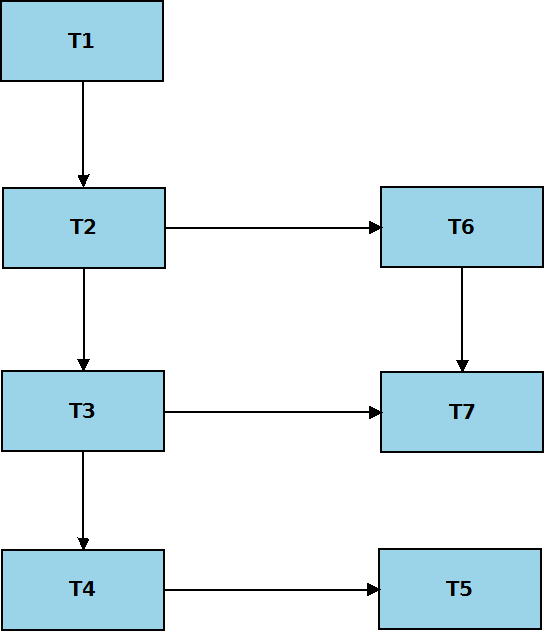
\includegraphics[width=0.5\textwidth]{dependencies.png}
\end{center}

In the following table, for each task, we are going to show the Duration, expressed in days, the Effort, measured in person-days, and the Dependencies with other tasks.
\begin{center}
	\begin{tabular}{c c c c}
		\hline
		\textbf{Task} & \textbf{Effort(person-days)} & \textbf{Duration(days)} & \textbf{Dependencies} \\
		\hline
		T1 & 146 & 30 & none \\
		T2 & 96 & 28 & T1 \\
		T3 & 43 & 35 & T1, T2 \\
		T4 & 66 & 21 & T1, T2 \\
		T5 & 50 & 66 & T1, T2, T3, T4 \\
		T6 & 10000 & 365 & T1, T2 \\
		T7 & 200 & 30 & T1, T2, T3, T4, T6  \\
		\hline
	\end{tabular}
\end{center}

This is the \textbf{Activity bar chart}, in which we provide a schedule in order to show when each task has to be done. It's alto highlighted the percentage of working already done until this moment.  
\begin{center}
	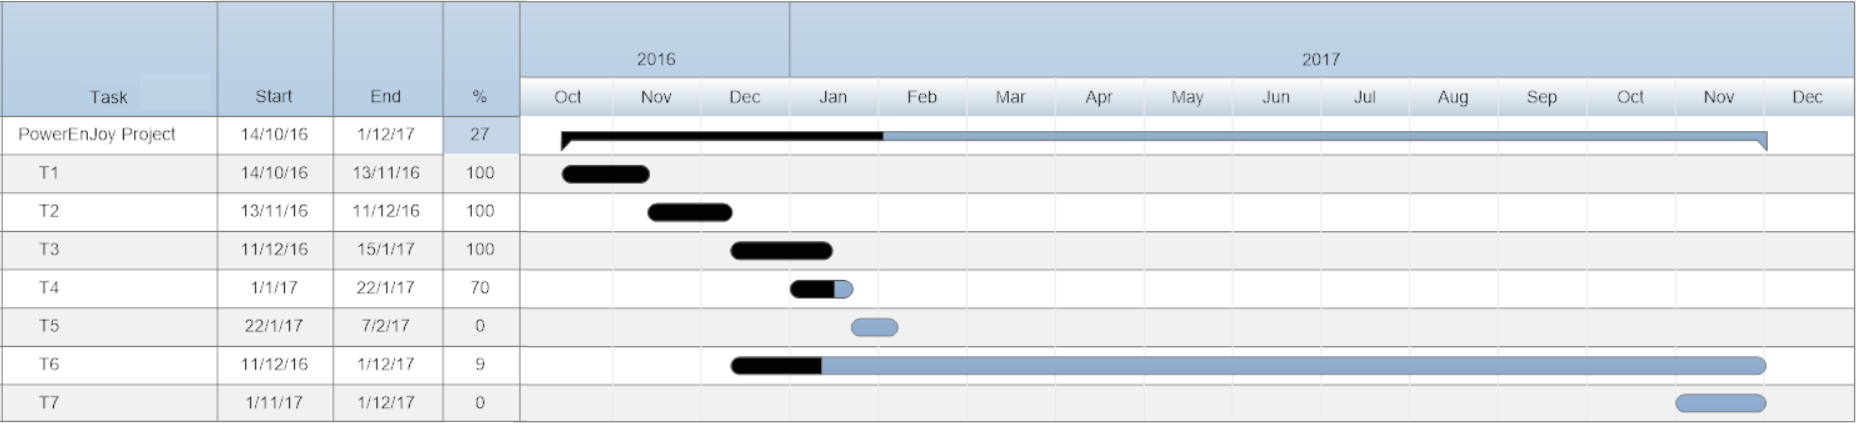
\includegraphics[width=\textwidth]{projectplan.png}
\end{center}

